\documentclass[svgnames,convert={density=300,size=720x600,outext=.png}]{standalone}
\usepackage{tikz,pgfplots,relsize}


\begin{document}
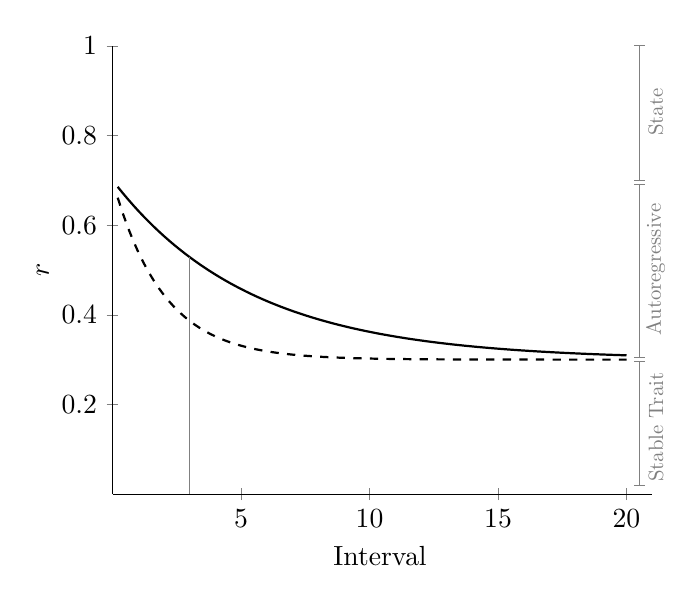
\begin{tikzpicture}

  \begin{axis}[
    axis lines=middle,
    axis line style={-},
    xmin=0, xmax=21, ymin=0, ymax=1,
    x label style={at={(axis description cs:0.6,-0.18), anchor=north}},
    y label style={at={(axis description cs:-0.1,.5)},rotate=90,anchor=south},
    ylabel=$r$,
    xlabel=Interval]
    \addplot[black, thick, samples=100, domain=.2:20] {.3 + .4*(.83^x)};
    \addplot[black, thick, dashed, samples=100, domain=.2:20] {.3 + .4*(.6^x)};
%    \addplot[lightgray, samples=100, domain=.2:20] {.3};
    \addplot +[gray, solid, mark=none] coordinates {(3,0) (3,.528)};
    \addplot +[gray, solid, mark=-] coordinates {(20.5,.02) (20.5,.295)};
    \addplot +[gray, solid, mark=-] coordinates {(20.5,.305) (20.5,.69)};
    \addplot +[gray, solid, mark=-] coordinates {(20.5,.70) (20.5,1)};    
  \end{axis}
  \node [gray, rotate=90, scale=.75] at (6.9,.85) {Stable Trait};
  \node [gray, rotate=90, scale=.75] at (6.9,2.85) {Autoregressive};
  \node [gray, rotate=90, scale=.75] at (6.9,4.85) {State};


\end{tikzpicture}

\end{document}  